\section{Introduction}
\label{sec:intro}

% Figure 1 is defined here, ahead of the text that cites it, so the two-column float lands at the top of page 2;
% defined later it was deferred past the section barrier (placeins) and left page 2 with an empty column.
\begin{figure*}[!t]
    \centering
    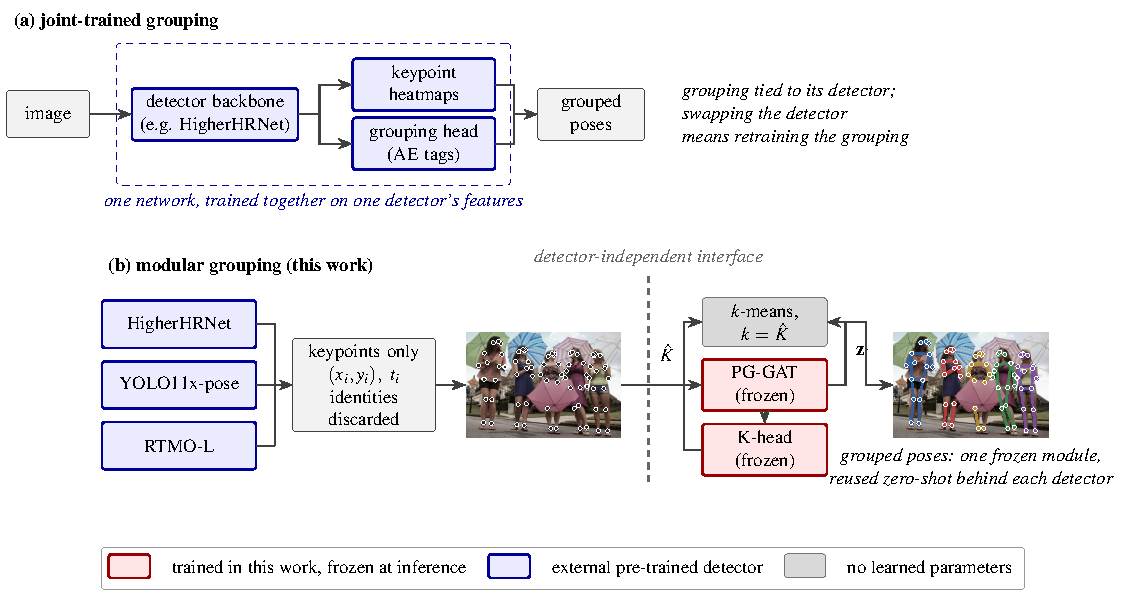
\includegraphics[width=\textwidth]{figures/concept_modular.pdf}
    \caption{Joint-trained versus modular grouping.
    (a) In established bottom-up methods the grouping head is trained with the keypoint detector
    on its internal features, which ties the grouping to that detector.
    (b) The modular pipeline exposes a keypoint-only interface shared by three detectors:
    PG-GAT embeds the detected keypoints, the K-head estimates the number of people $\hat K$,
    and $k$-means partitions the embeddings.
    PG-GAT and the K-head are trained once and remain frozen when the detector changes.
    Insets: COCO \texttt{val2017} image 281759 with the pooled HigherHRNet detections
    before grouping (grey) and after grouping by the modular pipeline (coloured by person).}
    \label{fig:concept}
\end{figure*}

% --- from chapter1_context.tex ---
In multi-person pose estimation, every person in an image must be localised at a fixed set of
anatomical joints, the seventeen joints of the COCO skeleton~\citep{lin2014coco}.
Bottom-up methods split the task into two stages:
a detector finds every keypoint in the image without assigning them to people,
and a grouping stage then assigns each detected keypoint to a person.
Keypoint detection is well studied,
and high-resolution convolutional backbones~\citep{sun2019hrnet,cheng2020higherhrnet},
transformer estimators~\citep{xu2022vitpose}
and human-centric foundation models~\citep{khirodkar2024sapiens} have raised localisation
accuracy on COCO to a point where further gains are small.
Grouping remains difficult for structural reasons.
The number of people is unknown at inference,
each person contributes at most one keypoint of each joint type,
occlusion and truncation remove keypoints without a predictable pattern,
and where people overlap in the image, same-type keypoints,
such as two left elbows, end up close together.

% --- from chapter1_context.tex and chapter1_research_gap.tex ---
In established bottom-up methods the grouping decision comes from a mechanism
trained jointly with the detector.
Part-affinity fields~\citep{cao2017openpose},
associative-embedding tags~\citep{newell2017associative,cheng2020higherhrnet},
centre-offset regression~\citep{geng2021dekr}
and end-to-end set prediction~\citep{shi2022petr} are the forms this mechanism takes,
and every one of them couples the grouping to a particular backbone.
The coupling buys accuracy at the cost of reuse: a grouping mechanism trained with one
detector cannot be detached and applied to the output of another.
The alternative, a grouping module that consumes keypoints from any detector,
has received comparatively little attention.
Among graph-based methods, hierarchical graph grouping~\citep{jin2020hgg} is trained jointly
with its detector,
and graph edge classification~\citep{maher2025gec} is detector-independent but classifies
pairs of keypoints rather than learning a representation of each keypoint.

This work develops the modular alternative and measures what the separation costs
(Figure~\ref{fig:concept}).
The interface between detector and grouping stage carries only detected keypoint
coordinates, visibility flags and joint types.
A graph attention network embeds the detected keypoints,
a small head, the K-head, estimates the number of people $\hat K$ from the embeddings,
and $k$-means partitions the embeddings into people.
The network and the head are trained once and remain frozen when the detector changes.
The accuracy lost to this separation is measured against a deliberately chosen
joint-trained reference:
the associative-embedding grouping of HigherHRNet~\citep{cheng2020higherhrnet},
evaluated on identical detections.
The same frozen module is then applied without retraining
to two further detectors from different architectural families.

% --- from chapter1_research_contributions.tex and summary.tex ---
The main contributions are as follows.
\begin{itemize}
    \item \textbf{PG-GAT}, a pose grouping graph attention network extending GATv2~\citep{brody2022gatv2}
    with a type-pair attention bias, skeleton-relative position encoding and same-type repulsion heads.
    It is trained on synthetic scenes and fine-tuned on COCO, and with a $k$-means read-out
    reaches 0.9715 pose grouping accuracy on COCO validation keypoints
    and 0.9591 on HigherHRNet detections, against 0.9847 for the detector's jointly trained
    associative embedding on the same detections.
    \item \textbf{Evidence that the embedding, not the grouping head, limits accuracy}: three learned
    grouping heads and ten modularity-based clustering variants did not improve on $k$-means
    once the model is applied to real data, while changes to the embedding produced the gains
    that transfer to real data. Attention analysis shows that PG-GAT directs its attention along
    same-person skeletal edges and away from same-type edges.
    \item \textbf{A measured cost of modularity}: with the K-head trained on the frozen embeddings,
    the pipeline needs no ground truth at inference. Applied zero-shot to YOLO11x-pose~\citep{ultralytics2024yolo11}
    and RTMO-L~\citep{lu2024rtmo}, it trails the native grouping of all three detectors
    by 0.020 to 0.022 on matched detections.
    At the system level the cost is 0.048 AP on identical joints,
    concentrated in scenes with more people than the synthetic training data contained.
    \item \textbf{Documented negative results}, in the configurations tested,
    for a hyperbolic embedding, a triplet-based graph primitive and appearance features,
    and the mechanism of failure in each case.
\end{itemize}